\section{Architecture Variants}
\label{sec:architectures}
%% ============================================================

\subsection{Standard Transformer (GPT)}

Each block applies:
\begin{align}
  \tilde{h} &= \mathrm{LN}(h), \label{eq:ln} \\
  \mathrm{attn} &= W_O \left[ \|_h\, \mathrm{softmax}\!\left(\tfrac{Q_h K_h^\top}{\sqrt{d_h}}\right) V_h \right], \\
  h &\leftarrow h + \mathrm{attn} + s_{\mathrm{ff}} \cdot \mathrm{FFN}(\tilde{h}). \label{eq:gpt_update}
\end{align}
where $Q_h = W_{Q,h}\tilde{h}$, $K_h = W_{K,h}\tilde{h}$, $V_h = W_{V,h}\tilde{h}$,
and $s_{\mathrm{ff}}$ is a learned scalar.

\subsection{Original Energy GPT (EGPT)}

EGPT uses $V_h{=}K_h$ as an \emph{efficiency decomposition}: flash attention is run on the
smaller head-space tensor $[A_h K_h]_t \in \mathbb{R}^{d_h}$, then the result is projected
back to hidden space by reusing $W_{Q,h}^\top$ (no extra parameters):
\begin{align}
  \mathrm{attn}_E &= \sum_h W_{Q,h}^\top A_h K_h, \quad A_h = \mathrm{softmax}\!\left(\tfrac{Q_h K_h^\top}{\sqrt{d_h}}\right), \\
  g &= \mathrm{attn}_E + s_{\mathrm{ff}} \cdot \mathrm{FFN}(\tilde{h}), \\
  h &\leftarrow h - W \cdot g. \label{eq:egpt_update}
\end{align}
The projection matrix $W$ (shape $d \times d$) acts as a preconditioner / policy.
Since $q_{h,t} = W_{Q,h} h_t$, the true gradient of the per-head energy
$E_h(h_t) = -\log\!\sum_s A_{h,ts}$ with respect to $h_t$ is exactly:
\begin{equation}
  \nabla_{h_t} E_h \;=\; W_{Q,h}^\top \,[A_h K_h]_t .
\end{equation}
\textbf{EGPT therefore computes the true energy gradient.}
The $V{=}K$ step is a factored representation that saves FLOPs during flash attention
(operating in $\mathbb{R}^{d_h}$ rather than $\mathbb{R}^{D}$) and is \emph{not} an
approximation.  The remaining component, $W \cdot g$, is an unconstrained $d{\times}d$
preconditioner applied after the (correct) gradient computation.

\textbf{Cost:} EGPT requires two additional $d{\times}d$ matrix multiplications
(proj\_attn, proj\_mlp) compared to GPT, and the $V{=}K$ attention kernel is slightly
more expensive than softmax attention with a separate $V$ projection.
At $d=768$, 12 layers: 359 vs.\ 321 MFLOPs/token.
At $d=1024$, 24 layers: 654 vs.\ 503 MFLOPs/token.

\subsection{Mixed-Head EGPT (V10, V11)}

A natural compromise: keep a fraction of heads as energy heads ($V{=}K$) and
the remaining heads as standard GPT heads ($V{=}W_V x$), sharing a single output projection:
\begin{align}
  \mathrm{attn}_{\mathrm{mix}} &= W_O \Bigl[
    \underbrace{\|_{h \in \mathcal{E}}\, A_h K_h}_{\text{energy heads}}
    \;\Big\|\;
    \underbrace{\|_{h \in \mathcal{G}}\, A_h V_h}_{\text{GPT heads}}
  \Bigr], \\
  h &\leftarrow h + \mathrm{attn}_{\mathrm{mix}} + s_{\mathrm{ff}} \cdot \mathrm{FFN}(\tilde{h}). \label{eq:mixed_update}
\end{align}
The block remains \emph{additive} (GPT-style update), not subtractive.
Mixed-head models can be implemented as a single attention kernel over all heads;
no separate forward pass is needed.
\textbf{Key limitation:} the shared $W_O$ applies an arbitrary learned projection to
energy-head outputs $A_h K_h$ --- it does \emph{not} use $W_{Q,h}^\top$ as EGPT does.
Therefore, unlike EGPT, V10 energy heads do \emph{not} compute the true energy gradient.

\subsection{Energy Gradient Output (EGrad, V27, V31)}

EGrad brings EGPT's $W_{Q,h}^\top$ output rule into the mixed-head context.
Recall that EGPT already computes the true gradient by reusing $W_Q^\top$;
the problem with V10 MixedHead is that its energy heads go through a shared $W_O$
that ignores the $W_{Q,h}^\top$ structure.
EGrad fixes this by giving energy heads their own $W_{Q,h}^\top$ output (no new params)
and GPT heads their own smaller $W_{O,\mathcal{G}}$.

The true gradient of the energy $E_h(h) = -\log \sum_i \exp(Q_h K_{h,i}^\top / \sqrt{d_h})$
with respect to $h$ at position $t$ is:
\begin{equation}
  \nabla_{h_t} E_h = W_{Q,h}^\top \bigl[ A_h K_h \bigr]_t, \label{eq:egrad}
\end{equation}
where $W_{Q,h}^\top \in \mathbb{R}^{D \times d_h}$ maps from head space back to
hidden dimension.
EGrad uses this true gradient as the energy-head output, while keeping the GPT-head
output and additive residual:
\begin{align}
  \mathrm{egrad}_h(t) &= W_{Q,h}^\top \bigl[ A_h K_h \bigr]_t, \\
  \mathrm{egrad\_out} &= \sum_h \mathrm{egrad}_h \quad \text{(summed across energy heads)}, \\
  h &\leftarrow h + \mathrm{egrad\_out} + W_{O,\mathcal{G}} \bigl[ \|_{h \in \mathcal{G}}\, A_h V_h \bigr]
       + s_{\mathrm{ff}} \cdot \mathrm{FFN}(\tilde{h}). \label{eq:egrad_update}
\end{align}
No extra projection matrix is required: the output-projection for energy heads is
$W_{Q,h}^\top$ (the transpose of the query projection), reused at no parameter cost.

\textbf{Recurrent extension.}
With layer reuse: $h^{(k+1)} = h^{(k)} + \mathrm{egrad\_out}^{(k)} + \ldots$ iterated
$n_k$ times per unique block $k$.  The total effective compute is
$\propto \sum_k n_k \times (4d^2 + 3d \cdot d_{\mathrm{int}})$.

\subsection{Energy Descent Output (EDesc, V28, V32)}

EDesc uses the mixed-head output (Eq.~\ref{eq:mixed_update}) as a gradient direction
and applies a \emph{subtractive} update, with no separate projection matrix
(\texttt{energy\_proj\_type: identity}):
\begin{equation}
  h \leftarrow h - \bigl(\mathrm{attn\_mix} + s_{\mathrm{ff}} \cdot \mathrm{FFN}(\tilde{h})\bigr). \label{eq:edesc_update}
\end{equation}
EDesc is simpler than EGrad: it keeps the $V{=}K$ energy heads but interprets
the whole block output as a descent direction.

\subsection{Comparison Table}

\begin{figure}[h]
  \centering
  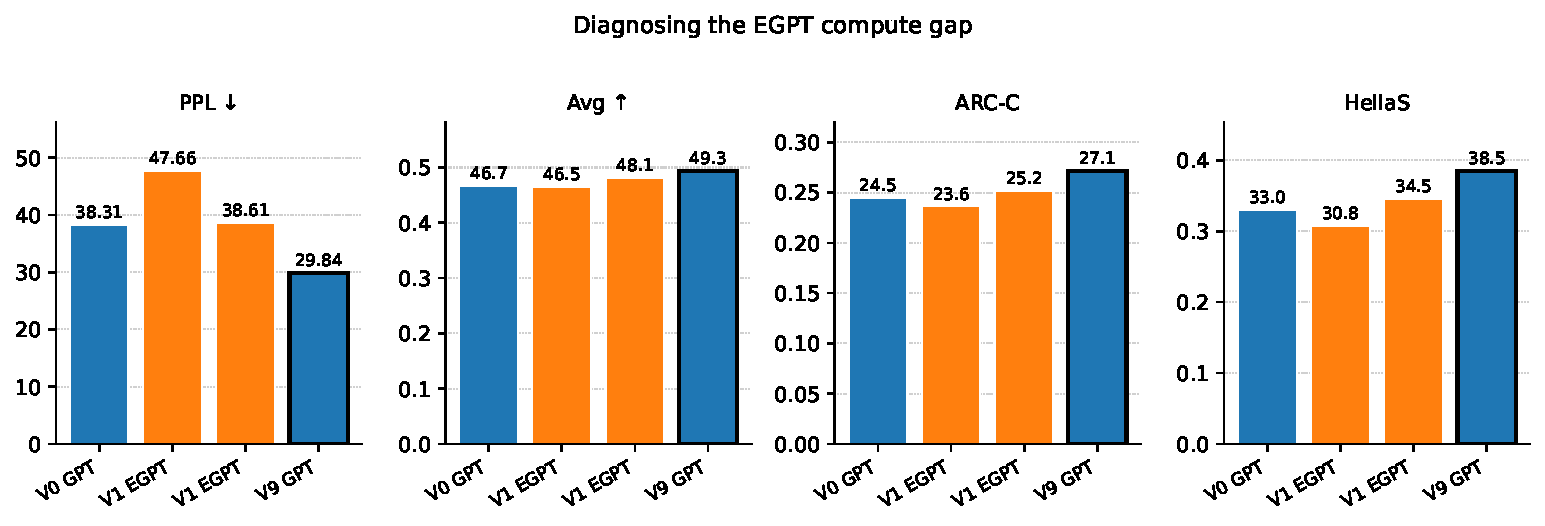
\includegraphics[width=\textwidth]{../results/multi-block-ablation/plots/bar_egpt_gap.pdf}
  \caption{Diagnosing the EGPT compute gap. Bars compare V0 GPT 12$\times$1 (162M, 321 MFLOPs/tok), V1 EGPT 12$\times$1 (143M, 359 MFLOPs/tok), V1 EGPT 24$\times$1 (400M, 755 MFLOPs/tok), and V9 GPT 24$\times$1 (354M, 503 MFLOPs/tok). EGPT trails GPT on PPL despite higher FLOPs.}
  \label{fig:bar_egpt_gap}
\end{figure}

\begin{figure}[h]
  \centering
  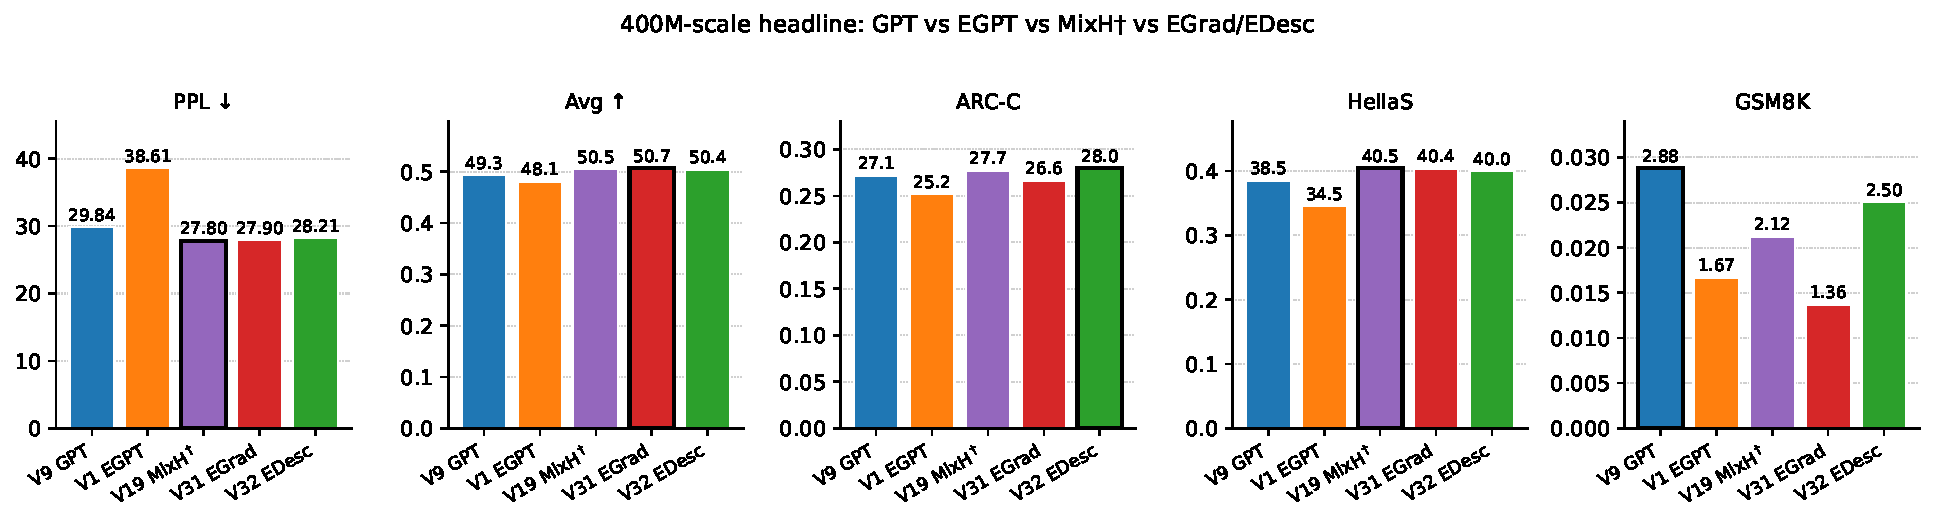
\includegraphics[width=\textwidth]{../results/multi-block-ablation/plots/bar_scaling.pdf}
  \caption{400M-scale headline. V19 MixH$^\dagger$, V31 EGrad, and V32 EDesc dominate the V9 GPT baseline on Avg accuracy and PPL at matched compute (503 MFLOPs/tok); V1 EGPT 24$\times$1 trails despite using more FLOPs.}
  \label{fig:bar_scaling}
\end{figure}

\begin{figure}[h]
  \centering
  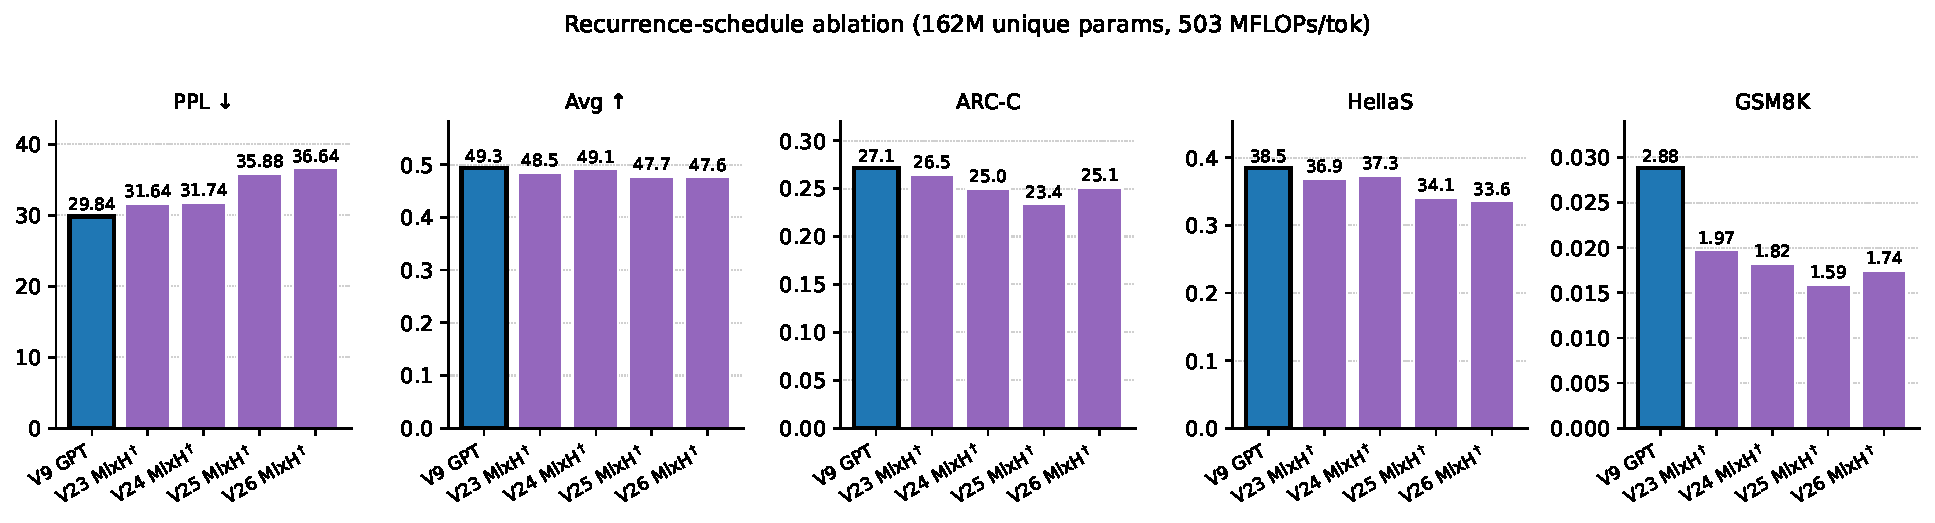
\includegraphics[width=\textwidth]{../results/multi-block-ablation/plots/bar_scaling_v25v26.pdf}
  \caption{Recurrence-schedule ablation (Mixed, 162M unique params, 503 MFLOPs/tok, 30k steps). V25 (uniform 6$\times$4) and V26 (back-loaded 6$\times$ramp) test whether more or non-uniform recurrence beats V23/V24 12$\times$2.}
  \label{fig:bar_scaling_v25v26}
\end{figure}

\begin{figure}[h]
  \centering
  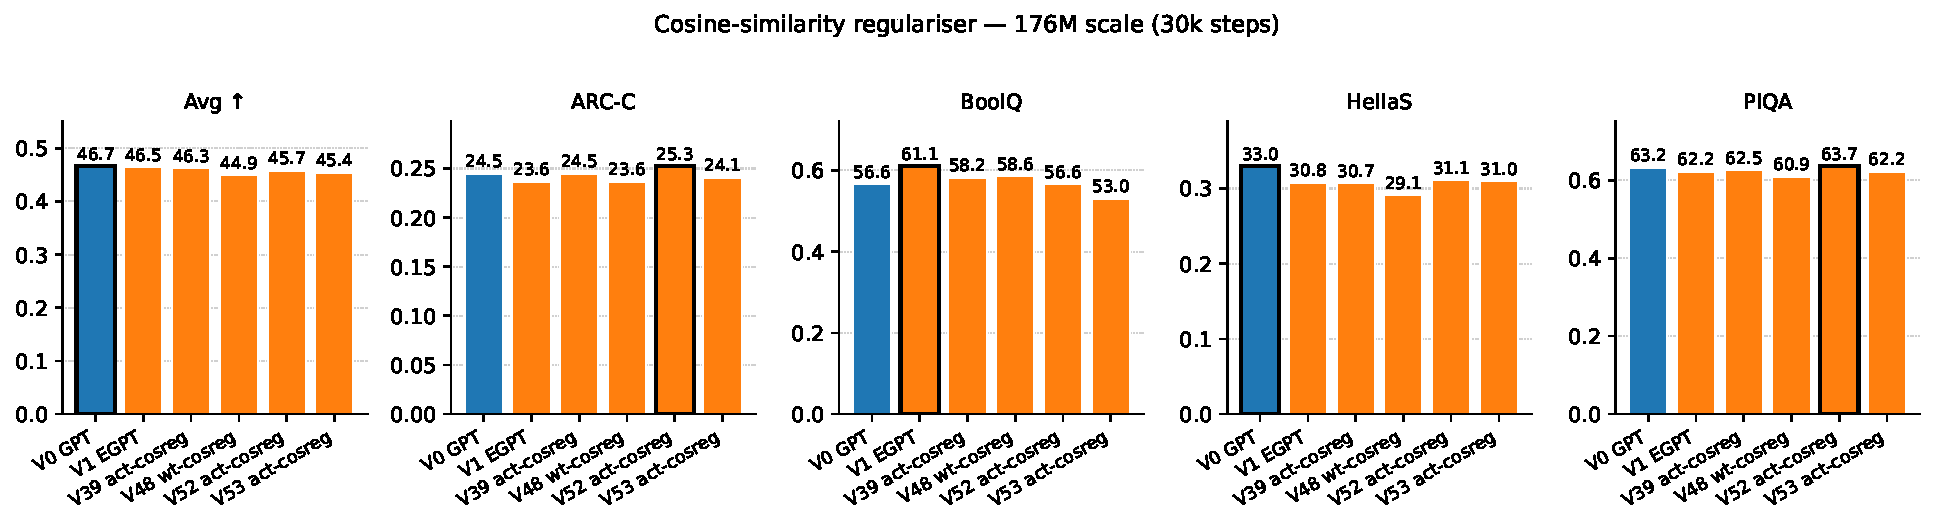
\includegraphics[width=\textwidth]{../results/multi-block-ablation/plots/bar_cosreg_benchmarks.pdf}
  \caption{Cosine-similarity regulariser performance (176M, 30k steps).
  Light cosreg ($\lambda{=}0.01$, V39 act / V48 wt) is roughly free; the
  stronger variants V52 ($\lambda{=}0.1$) and V53 (cosine ramp $0{\to}1.0$)
  cost $\approx$0.8--1.1 accuracy points on average vs V1 EGPT.
  V52 takes the best ARC-C (25.3) and PIQA (63.7), V53 leads on ARC-E among
  EGPT variants. V48 (weight-cosreg) loses the most ($-$1.6 vs V1).
  Avg uses the canonical 10-task set (\texttt{acc\_norm} where applicable);
  per-task numbers also use \texttt{acc\_norm} so they match the headline tables.
  Full layer-alignment heatmaps and consecutive-pair cosim plots for this sweep
  (cluster job 20260426) are pending.}
  \label{fig:bar_cosreg_benchmarks}
\end{figure}

\begin{table}[h]
\centering
\caption{Architecture comparison. All use shared $W_O$ across heads within a block.
  ``Additive'' = residual $+$; ``Descent'' = residual $-$.
  EGrad uses $W_Q^\top$ as energy head output projection (no new params).}
\label{tab:arch_compare}
\begin{tabular}{lllll}
\toprule
\textbf{Model} & \textbf{Attn output} & \textbf{Block update} & \textbf{New params} & \textbf{Extra FLOPs} \\
\midrule
GPT         & $A V$ (std)       & Additive    & $W_V$ per head      & none \\
EGPT        & $A K$ (energy)    & Descent     & proj\_attn, proj\_mlp & $2d^2$ per block \\
Mixed (V10) & $A K$ + $A V$     & Additive    & $W_V$ for GPT heads & none vs.\ GPT \\
EGrad (V27) & $W_Q^\top A K$ + $A V$ & Additive & none (reuse $W_Q$) & small \\
EDesc (V28) & $A K$ + $A V$     & Descent     & none                 & none \\
\bottomrule
\end{tabular}
\end{table}

%% ============================================================
